\chapter{Grundlagen der medizinischen Schrei-Forschung}

\section{Schmerz Scores}
Bei erwachsenen Menschen wird der Schmerzgrad typischerweise durch eine Selbsteinschätzung des Patienten unter der Leitung gezielter Fragen des Arztes vorgenommen. Bei Kindern unter 3 Jahren ist diese Selbsteinschätzung nicht möglich. Schmerz drückt sich in Veränderungen des psychologischen, körperlichen und biochemischen Verhaltens des Säuglings aus. Die für den Arzt am leichtesten feststellbaren Verhaltensänderungen sind von außen wahrnehmbaren Merkmale, wie zum Beispiel ein Verkrampfen des Gesichtsausdrucks, erhöhte Körperbewegungen oder lang anhaltendes Weinen. Um eine weitesgehend objektive Schmerzfeststellung zu ermöglichen, wurden sogenannte \emph{Pain-Scores} entwickelt, die durch ein Punktesystem den insgesamten Schmerzgrad des Babies quantifizieren.\cite{PainAssessment01} Es existieren \emph{eindimensionale} Pain-Scores, die den Schmerz nur Aufgrund der Beobachtung eines Merkmals beurteilen, so wie beispielsweise die reine Beurteilung des Gesichtsausdruckes. \emph{Mehrdimensionale} (auch \emph{ multimodale}) Pain-Scores beziehen mehrere Faktoren in das Scoring mit ein.\cite{PainAssessment02}. Tabelle \ref{tab:nips} zeigt das Scoring-System \glqq Neonatal Infant Pain Scale\grqq{}(NIPS) als Beispiel für eine multimodale Pain-Score. Der Säugling wird anhand der aufgeführten Kategorien bewertet und alle vergebenen Punkte aufsummiert. Ein insgesamter Wert von $>3$ zeigt Schmerz an, ein Wert von $>4$ großen Schmerz.\cite{nips}

\begin{table}[h]
	\footnotesize
	\centering
	\caption{NIPS-Scoring}
	\label{tab:nips}
	\begin{tabular}{@{}cccc@{}}
		\toprule
		\textbf{NIPS}     & \textbf{0 points} & \textbf{1 point}     & \textbf{2 points} \\ \midrule
		Facial Expr. & Relaxed           & Contracted           & -                 \\
		Cry               & Absent            & Mumbling             & Vigorous          \\
		Breathing         & Relaxed           & Different than basal & -                 \\
		Arms              & Relaxed           & flexed/stretched     & -                 \\
		Legs              & Relaxed           & flexed/stretched     & -                 \\
		Alertness         & Sleeping          & uncomfortable        & -                 \\ \bottomrule
	\end{tabular}
\end{table}


In den meisten mehrdimensionalen Scoring-Systeme werden die Schreigeräusche mit einbezogen. Tabelle \ref{tab:painscores} zeigt eine Übersicht über eine ausgewählte Menge an multimodalen Pain-Scores. Alle Pain-Scores sind für Kleinkinder bis 3 Jahren gedacht. In der Übersicht wird nicht wiedergegeben, welche weiteren Merkmale jeweils in das Scoring mit einbezogen werden, oder welche Insgesamtpunktzahlen auf welche Schmerzintensität hinweisen. Es soll an dieser Stelle nur verdeutlicht werden, welche unterschiedlichen Ansätze zur Bewertung des Schreiens aus medizinischer Sicht im Zusammenhang mit Pain-Scores existieren. Folgende Beobachtungen lassen sich aus der Übersicht ziehen:

\begin{enumerate}

\item Die zu beobachtenden Eigenschaften des Weinens werden mit subjektiv behafteten Werten charakterisiert. Beispielsweise wird im N-PASS-System ist ein Schmerz-Schrei als \glqq High-pitched or silent-continuous crying\grqq{} beschrieben. Es wird nicht fest definiert, was als \glqq crying\grqq{} gilt oder welche Tonhöhe als \glqq high-pitched\grqq{} ist. Auch die Erstquellen geben keine festen Definitionen.

\item Es gibt verschiedene Ansätze zur Bewertung des Weinens. Bei CRIE ist die Tonhöhe, bei BIIP die Länge und bei COMFORT die Art des Weinens entscheidend.

\item Die Beschreibungen sind kurz und prägnant gehalten, der Arzt hat in keinem der Modelle auf mehr als drei Parameter des Schreiens zu achten. Die Begründung liegt darin, dass bei allen Modellen a.) das Schreien nur eines von mehreren Faktoren ist, und b.) Die Schmerzbestimmung in einem vorgegebenen Zeitrahmen durchführbare sein muss.

\end{enumerate}

%\begin{table}[H]
%	\centering
	\begin{longtable}{@{}lll@{}}
	
%	\begin{tabular}{@{}lll@{}}
		\toprule
		\textbf{System} & \textbf{P.} & \textbf{Description}                                                                                \\ \midrule
		FLACC\cite{flacc}           & 0           & No cry (awake or asleep)                                                                            \\
		& 1           & Moans or whimpers; occasional complaint                                                             \\
		& 2           & \begin{tabular}[c]{@{}l@{}}Crying steadily, screams or sobs, \\ frequent complaints\end{tabular}    \\\midrule
		N-PASS\cite{npass}          & -2          & No cry with painful stimul                                                                          \\
		& -1          & \begin{tabular}[c]{@{}l@{}}Moans or cries minimally \\ with painful stimuli\end{tabular}            \\
		& 0           & Appropiate Crying                                                                                   \\
		& 1           & \begin{tabular}[c]{@{}l@{}}Irritable or Crying at Intervals.\\ Consolable\end{tabular}                                                        \\
		& 2           & \begin{tabular}[c]{@{}l@{}}High-pitched or silent-continuous crying. \\ Not consolable\end{tabular} \\\midrule
		BIIP\cite{BIIP}            & 0           & No Crying                                                                                           \\
		& 1           & Crying \textless 2 minutes                                                                          \\
		& 2           & Crying \textgreater 2 minutes                                                                       \\
		& 3           & Shrill Crying \textgreater 2 minutes                                                                \\\midrule
		CRIES\cite{cries}            & 0           & If no cry or cry which is not high pitched                                                          \\
		& 1           & \begin{tabular}[c]{@{}l@{}}If cry high pitched but baby \\ is easily consoled\end{tabular}          \\
		& 2           & \begin{tabular}[c]{@{}l@{}}If cry is high pitched and baby \\ is inconsolable\end{tabular}          \\\midrule
		COVERS\cite{covers}          & 0           & No Cry                                                                                              \\
		& 1           & High-Pitched or visibly crying                                                                      \\
		& 2           & Inconsolable or difficult to soothe                                                                 \\\midrule
		PAT\cite{pat}             & 0           & No Cry                                                                                              \\
		& 1           & Cry                                                                                                 \\\midrule
		DAN\cite{dan}             & 0           & Moans Briefly                                                                                       \\
		& 1           & Intermittent Crying                                                                                 \\
		& 2           & Long-Lasting Crying, Continuous howl                                                                \\\midrule
		COMFORT\cite{comfort}         & 0           & No crying                                                                                           \\
		& 1           & Sobbing or gasping                                                                                  \\
		& 2           & Moaning                                                                                             \\
		& 3           & Crying                                                                                              \\
		& 4           & Screaming                                                                                           \\\midrule
		MBPS\cite{mbps}            & 0           & Laughing or giggling                                                                                \\
		& 1           & Not Crying                                                                                          \\
		& 2           & \begin{tabular}[c]{@{}l@{}}Moaning quiet vocalizing gentle or \\ whimpering cry\end{tabular}        \\
		& 3           & Full lunged cry or sobbing                                                                          \\
		& 4           & Full lunged cry more than baseline cry                                                              \\ \bottomrule
	%\end{tabular}
			\caption{Übersicht über Pain-Scores}
	\label{tab:painscores}
	\end{longtable}
%\end{table}

\section{Schmerz-Schrei aus medizinischer Sicht}

Die Frage ist: Woher kommen diese unterschiedlichen Bewertungen des Weinens in Tabelle \ref{tab:painscores}? Gibt es eine Pain-Score, die aus wissenchaftlicher Sicht \glqq recht hat\grqq ? Dieser Fragestellung unterliegen unterliegen zwei grundlegendere Fragen: 1.) Ist es überhaupt möglich, anhand der akustischen Eigenschaften den Grund für den Schrei abzuleiten, also beispielsweise Hunger, Einsamkeit oder Schmerz? Anders formuliert: Gibt es überhaupt so etwas wie einen Schmerz-Schrei? 2.) Ist es möglich, anhand der akustischen Eigenschaften den Schweregrad des Unwohlseins abzuleiten (also beispielsweise den Grad des Schrei-Versursachenden Schmerzes)?

Die Annahme, dass es möglich ist, aus dem Schreien den Grund abzuleiten, wird als \glqq Cry-Types Hypothesis\grqq{} bezeichnet. Die berühmtesten Befürworter dieser Hypothese ist eine skandinavische Forschungsgruppe, auch bezeichnet als \glqq Scandinavian Cry-Group\grqq , die diese Idee in dem Buch \glqq Infant Crying: Theoretical and Research Perspectives\grqq \cite{crygroup} publik machte. Die Annahme ist, dass die verschiedenen Ursachen \emph{Hunger, Freude, Schmerz, Geburt und Anderes} klare Unterschiede hinsichtlich ihrer akustischen Merkmale aufweisen, welche an einem Spektogramm ablesbar seien. Entsprechende Beispiele werden in dem Buch gegeben. Nur einige Jahre Später zeigte Müller et al \cite{cryisnoise} in einem Paper, dass bei leichter Veränderung der Bedingungen der Experimente die Unterscheidung nicht möglich ist. Die Gegenhypothese ist, dass Weinen \glqq nichts als undifferenziertes Rauschen\grqq{} sei. 50 Jahre später liegt kein anerkannter Beweis für die eine oder andere Hypothese vor. Es gibt nur starke Hinweise dafür, dass die Plötzlichkeit des Eintretens des Schreigrundes hörbar ist. Ein plötzliches Ereignis, wie ein Nadelstich oder ein lautes Geräuch, führen auch zu einem plötzlich beginnenden Schreien. Ein langsam einretendes Ereignis, wie ein langsam immer stärker werdender physischer Schmerz oder langsam eintretender Hunger führen auch zu einem langsam eintretenden Weinen. Da keine Einigung herrscht, wird empfohlen, den Grund aus dem Kontext abzuleiten.\cite{signal}

Die Zweite Frage nach der Ableitung der Stärke des Unwohlseins aus den akustischen Eigenschaften des Geschreis wird in der Fachsprache unter dem Begriff \emph{Cry as a graded Signal} subsumiert. Je \glqq stärker\grqq{} das Weinen, desto höher das Unwohlsein (\emph{Level of Distress (LoD)}) des Säuglings. Tatsächlich bemessen wird dabei der von dem Beobachter vermutete Grad des Unwohlsein des Babies, und nicht der tatsächliche Grad, da dieser ohne die Möglichkeit der direkten Befragung des Kindes nie mit absoluter Sicherheit bestimmt werden kann. Dieser vermutete LoD  wird entweder durch das subjektive Empfinden der Beobachter oder durch Pain-Scores festgestellt. Ein hohes Level of Distress hat vor allem eine schnelle Reaktion der Aufsichtspersonen zur Beruhigung des Babies zur Folge, womit dem Geschrei eine Art Alarm-Funktion zukommt. Es gibt starke Hinweise darauf, dass das Level of Distress anhand objektiv messbarer Eigenschaften des Audiosignals bestimmt werden kann. So herrscht beispielsweise weitesgehend Einigung darüber, dass ein \glqq lang\grqq{} anhaltendes Geschrei auf einen hohen Level of Distress hinweist. Insofern aus dem Kontext des Schreiens Schmerz als wahrscheinlichste Ursache eingegrenzt werden kann, kann aus einem hohen Level of Distress ein hoher Schmerz abgeleitet werden. \cite{signal} und \cite{lod}

Es herrscht wiederum keine Einigung darüber, welche akustischen Eigenschaften im Detail ein hohes Level of Distress anzeigen. Carlo V Bellieni et al \cite{dan} haben festgestellt, dass bei sehr hohem Schmerz in Bezug auf die DAN-Scala (siehe Tabelle \ref{tab:painscores}) die Tonhöhe des Geschreis steigt. Qiaobing Xie et al \cite{lod} haben festgestellt, dass häufiges und \glqq verzerrtes\grqq{} Schreien (ohne feststellbares Grundfrequenz, da der Ton stimmlos erzeugt wird)  auf einen hohen Level of Distress hinweist.\cite{signal} Diese Uneinigkeit hat wahrscheinlich zu den verschiedenen Bewertungen in den Pain-Scores geführt. \ref{tab:painscores}.

\section{Phyisio-Akustische Modellierung des Weinens}
\label{sec:acousticModel}

Das Ziel dieses Kapitels ist die Schaffung eines einheitlichen Vokabulares, auf den sich bezogen wird, um das Schreien eines Babys zu beschreiben. Die hier vorgestellten Begriffe stammen sowohl aus dem Buch \glqq A Physioacoustic Model of the Infant Cry \grqq{} H Golub und M Corwin \cite{cryModel} als auch aus dem Paper \glqq Rythmic organization of the Sound of Infant Cry \grqq{} von Zeskind et al.\cite{rythmic}


Die Lautäußerung eines Neugeborenen, umgangssprachlich auch als \glqq Weinen\grqq{} oder \glqq Schreien\grqq{} bezeichnet, lässt sich im allgemeinen beschreiben als das \glqq rythmische Wiederholen eines beim ausatmen erzeugen Geräusches, einer kurzen Pause, einem Einatmungs-Geräusch, einer zweiten Pause, und dem erneuten Beginnen des Ausatmungs-Geräusches.\grqq \cite{wolff}.

Das Vokabular, welches insbesondere von H Golub und M Corwin geschaffen wurde, ist sehr umfassend. An dieser Stelle wird eine Auswahl grundlegender Begrifflichkeiten vorgestellt, die in dieser Arbeit gebraucht werden. Sie werden in Abbildung \ref{img:cryVocabulary} veranschaulicht.

\begin{description}
	\item[Expiration] beschreibt den Klang, der bei einem einzelnen, ununterbrochenem Ausatmen mit Aktivierung der Stimmbänder durch das Baby erzeugt wird. \cite{rythmic}. Der von Golub et al \cite{cryModel} verwendete Begriff \textbf{Cry-Unit} wird in dieser Arbeit synonym verwendet. Umgangssprachlich ist handelt es sich um einen einzelnen, ununterbrochenen \emph{Schrei}.
	\item[Inspiration] beschreibt den Klang, der beim Einatmen durch das Baby erzeugt wird.
	\item[Burst] beshreibt die Einheit von einer Expiration und der darauf folgenden Inspiration. Das heisst, dass die zeitliche Dauer eines Bursts sowohl das Expiration-Geräusch, das Inspiration-Geräusch als auch die beiden Pausen zwischen diesen Geräuschen umfasst. Praktisch ergibt sich das Problem, dass vor allem bei stärkerem Hintergrundrauschen die Inspiration-Geräusche häufig weder hörbar noch auf dem Spektrogramm erkennbar sind. Daher wird die Zeitdauer eines Bursts oder Cry-Unit vom Beginn einer Expiration bis zum Beginn der darauf folgenden Expiration definiert und somit allein von den Expirations auf die Bursts geschlossen. Implizit wird somit eine Inspiration zwischen zwei Expirations angenommen.
	\item[Cry] die insgesamte klangliche Antwort zu einem spezifischen Stimulus. Eine Gruppe mehrerer Cry-Units.\cite{cryModel} In dieser Arbeit wird ein \emph{Cry} als \textbf{Cry-Segment} bezeichnet, um Verwechslungen zu vermeiden.
\end{description}

\begin{figure}
	\centering
	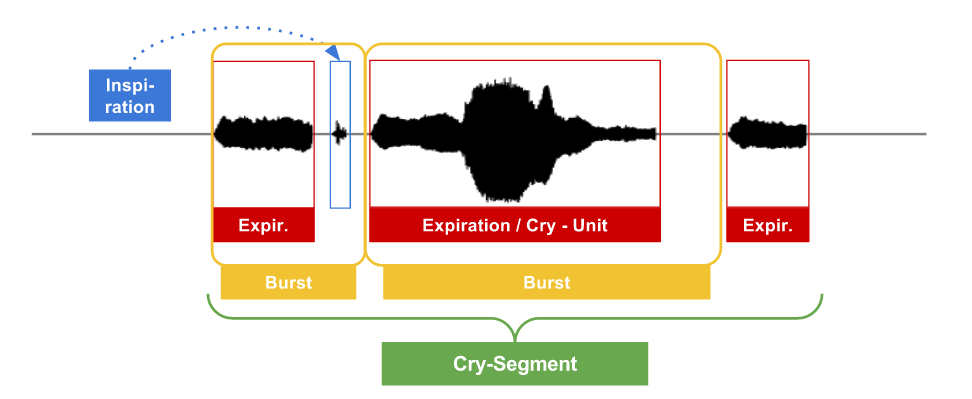
\includegraphics[width=0.7\textwidth]{bilder/cryVoc02.png}
	\caption{Veranschaulichung des Grundvokabulars}
	\label{img:cryVocabulary}
\end{figure}

Weiterhin wurden von H Golub und M Corwin \cite{cryModel} Cry-Units in eine der folgenden drei Kategorien eingeführt:

\begin{description}
	\item[Phonation] beschreibt eine Cry-Unit mit einer \glqq vollen Vibration der Stimmbänder\grqq{} mit einer Grundfrequenz zwischen 250 und \SI{700}{\hertz}. Entspricht umgangssprachlich einem Weinen mit einem \glqq klaren, hörbaren Ton\grqq{}.
	\item[Hyper-Phonation] beschreibt eine Cry-Unit mit einer \glqq falsetto-artigem Vibration der Stimmbänder\grqq{} mit einer Grundfrequenz zwischen 1000 und \SI{2000}{\hertz}. Entspricht umgangssprachlich einem Weinen mit einem \glqq sehr hohen, aber klaren, hörbaren Ton\grqq{}.
	\item[Dysphonation] beschreibt eine Cry-Unit ohne klar feststellbare Tonhöhe, produziert durch Turbulenzen an den Stimmbändern. Entspricht umgangsprachlichen dem \glqq Brüllen oder Krächzen\grqq{}.
\end{description}

Eine Cry-Unit gehört dabei mindestens einer dieser Kategorien an, kann aber auch in seinem zeitlichen Verlauf die Kategorie wechseln. H Golub und M Corwin \cite{cryModel} stellen weiterhin eine Reihe an charakteristischen Eigenschaften vor, die in Bezug auf ein Cry-Segment berechnet werden. 

\begin{description}
	\item[Latency-Period] beschreibt die Dauer zwischen dem zufügen eines Schmerz-Stimulus und dem beginn des ersten Cry-Bursts des Segmentes
	\item[Duration] beschreibt die insgesamte Zeitdauer des Cry-Segmentes. Es wird keine genaue Definition gegeben, wodurch Beginn und Ende definiert werden. Das Segment endet dort, wo es \glqq scheint, aufzuhören\grqq{}.
	\item[Maximum-Pitch] beschreibt die höchste festgetellte Grunfrequenz des Segmentes. 
\end{description}

... und viele weitere, die in \cite{cryModel} nachgelesen werden können, aus Platzgründen an dieser Stelle jedoch nicht vollständig genannt werden.